\section{Related Work}
\label{sec:related}

\emph{We don't do our studies in a vacuum.  It would be hard to breathe.  Moreover, it would be hard for the swallows to fly.  As such, we must begin any study--a class project, a lab, a research project, or the development of a new product--with a careful analysis of the related work that was done previously.  It conveys professional maturity to cite the relevant work and to put it into proper context with your own work.  But just as importantly, we don't want to do needless work--if we can borrow from others, we should.  And of course any such borrowing must bear a proper citation of their work.  As such, in this section, you should discuss principles, theory, and prior work that has a direct relationship to your work. You can and should make reference to relevant principles and theory from your past labs without repeating that material in your write-up. Think about what you are being asked to measure.}

In understanding the relationship between bandwidth and air-speed, we must understand the system required to transmit the data. The AtSwallow128A flies with a carrier frequency of 2.4GFlaps/s. Per flight, a typical packet size of 500 grams can be transferred. However, 50 grams of this packet must be dedicated to overhead to ensure the packet's validity and to fasten it to the bird. Figure~\ref{fig:packet} shows typical packet overhead for a bird this size. Thus, only 450 grams of each transfer can be considered useful data.

Bonomi's well-regarded work in fog computing work \cite{Bonomi2012} relates to our study because fog can be an especially important factor in conducting predictable flight studies.  We note that Bonomi's work did not anticipate the specific case of African swallows and, as such, we seek to extend his work.  Athreya \cite{Athreya2014} considers the energy effects of conveying packets using mesh networking.  It is our strong belief that the replacement of Athreya's wireless links with swallows, generally, and African swallows in particular, would result in a much richer opportunity for understanding the energy cost of conveying packets across different air interface types.  We seek such a broadened understanding.

\begin{figure}[h]
\centering
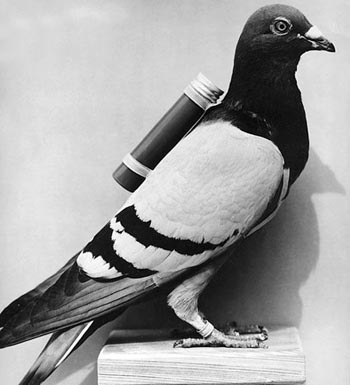
\includegraphics[width=0.3\textwidth]{carrier_pigeon}
\caption{A typical packet on a bird.}
\label{fig:packet}
\end{figure}

The air-speed of the bird likewise depends on many factors, such as wind velocity, gravitational effects, and the phase of the moon. However, packet weight has a first-order effect on air-speed, as much as 90\%. We thus only examine the effect of packet weight in this experiment while controlling the other factors.

A bird's power consumption is related to its flight weight by Equation~\ref{eqn:powerconsumption}.

\begin{equation}
\label{eqn:powerconsumption}
P = 0.45 W + g f_{flight}
\end{equation}

where $P$ is the power consumed [worms/s], $W$ is the weight [n], $g$ is the gravitational constant, and $f_{flight}$ is the frequency of flight [$flights/sec$].

Equation~\ref{eqn:airspeed} relates power consumption to air-speed.

\begin{equation}
\label{eqn:airspeed}
P = S_{air}^2
\end{equation}

Given this relationship, we expect that an increase in weight will result in a inverse-square decrease in airspeed; that is, the two have an inverse quadratic relationship. If  this prediction can be validated experimentally, we can be confident that the inverse-square law alone can be used to model the African swallow's speed as a function of weight.

